\documentclass[conference]{IEEEtran}

\IEEEoverridecommandlockouts
% The preceding line is only needed to identify funding in the first footnote. If that is unneeded, please comment it out.
\usepackage{cite}
\usepackage{amsmath,amssymb,amsfonts}
% \usepackage{algorithm}
\usepackage[ruled,vlined]{algorithm2e}
% \usepackage{algorithmic}
\usepackage{algpseudocode}
\usepackage{graphicx}
\usepackage{textcomp}
\usepackage{xcolor}
\usepackage{booktabs}
\usepackage{array}
\usepackage{makecell}
\usepackage{multirow}
\usepackage{subfig}


\usepackage{amsmath}

\def\BibTeX{{\rm B\kern-.05em{\sc i\kern-.025em b}\kern-.08em
    T\kern-.1667em\lower.7ex\hbox{E}\kern-.125emX}}
\begin{document}

\title{SLNN-Assisted Decoding of a 7/9-Rate Sparse Code for Reliable STT-MRAM}

% {\footnotesize \textsuperscript{*}Note: Sub-titles are not captured in Xplore and
% should not be used}
% \thanks{Identify applicable funding agency here. If none, delete this.}
% }

\author{
\IEEEauthorblockN{
Nhon Quang Nguyen,
Huy Vinh Giang,
Thanh-Loc Nguyen-Van,
Tan Do-Duy
}

\IEEEauthorblockA{Ho Chi Minh City University of Technology and Engineering (HCM-UTE), Vietnam
}

}

\maketitle

\begin{abstract}

Spin-transfer torque magnetic random-access memory (STT-MRAM) is a promising non-volatile memory technology, but its reliability is limited by asymmetric write failures and read errors. This paper proposes a single-label neural network (SLNN)-based decoder for the existing 7/9-rate sparse code to replace the conventional maximum-likelihood (ML) decoder. The proposed decoder reformulates sparse decoding as a 128-class single-label classification problem, enabling direct learning of the nonlinear mapping between noisy received vectors and valid sparse codewords using the soft information of the received signals. A lightweight feedforward neural network is employed to maintain low implementation complexity. Simulation results show that the proposed decoder reduces both bit error rate (BER) and frame error rate (FER) by approximately 60\% on average compared with the ML decoder under various channel conditions, demonstrating the effectiveness of neural-assisted sparse decoding for improving STT-MRAM reliability.

\end{abstract}

\begin{IEEEkeywords}
Spin-transfer torque magnetic random-access memory (STT-MRAM), sparse codes, neural network, soft-decision decoding.
\end{IEEEkeywords}



\section{Introduction}

Spin-Transfer Torque Magnetic Random Access Memory (STT-MRAM) is a promising non-volatile memory technology because of its high density, fast read/write operations, high endurance, and suitability for emerging Internet of Things (IoT) and artificial intelligence (AI) applications \cite{girard2020survey}. However, ensuring reliable data storage remains a major challenge, as both write- and read-induced errors become increasingly severe with continued technology scaling \cite{hemaram2025asymmetric}.

The reliability degradation of STT-MRAM mainly originates from the stochastic switching behavior of magnetic tunnel junctions (MTJs). Process variations in MTJ geometry and resistance alter the switching current distribution, causing cell-to-cell variability. Since practical memory systems employ a fixed write pulse width, some MTJs fail to complete switching within the allocated write duration, resulting in write failures. Thermal fluctuations, read disturbance, and manufacturing imperfections further aggravate these effects, making reliability enhancement increasingly difficult as device dimensions continue to shrink \cite{wu2020survey}.

To mitigate these reliability issues, channel coding techniques have been widely adopted for memory protection. Existing approaches include constrained coding, error-correcting codes (ECCs), and their combination \cite{nguyen2026error}. While ECCs, such as Hamming and BCH codes, provide reliable error correction, they cannot fully exploit the asymmetric write-error characteristic of STT-MRAM, where the $(0 \rightarrow 1)$ write-error probability can be up to three orders of magnitude higher than that of $(1 \rightarrow 0)$ transitions \cite{hemaram2025asymmetric}. To address this asymmetry, the 7/9-rate sparse code proposed in \cite{nguyen2021design} reduces the number of stored ``1'' bits and consequently the number of vulnerable $(0 \rightarrow 1)$ write transitions. However, its decoder is conventionally implemented using maximum-likelihood (ML) decoding, whose distance-based hard-decision operation cannot effectively exploit the reliability information of the read signals.

The original 7/9-rate sparse code proposed in \cite{nguyen2021design} employs a conventional maximum-likelihood (ML) decoder without neural assistance. Subsequent studies introduced neural networks only for channel detection. Specifically, Nguyen \textit{et al.}~\cite{nguyen2021performance} proposed an RNN-based detector, while Nguyen \textit{et al.}~\cite{nguyen2023neural} developed an MLP-based detector to improve sensing reliability prior to sparse decoding. Nevertheless, the final sparse decoding stage still relies on the conventional ML decoder, limiting the overall decoding performance. Motivated by this limitation, this paper develops a Single-Label Neural Network (SLNN)-based decoder for the existing 7/9-rate sparse code. 
To address this limitation, the proposed SLNN-based decoder replaces the conventional ML decoder and directly learns the nonlinear mapping from noisy received vectors to valid sparse codewords using the soft information of the received signals. By introducing neural learning into the sparse decoding stage, the proposed decoder improves sparse decoding accuracy while maintaining low decoding complexity, thereby enhancing the reliability of STT-MRAM under asymmetric write and read errors.


% \begin{table}[!t]
% \centering
% \caption{Comparison with existing neural-assisted reliability enhancement schemes for STT-MRAM.}
% \label{tab:comparison}

% \footnotesize
% \setlength{\tabcolsep}{3pt}
% \renewcommand{\arraystretch}{1.15}

% \begin{tabular}{|p{2cm}|p{2cm}|p{2cm}|p{2cm}|}
% \hline
% \textbf{Paper} &
% \textbf{7/9-rate Sparse Code} &
% {\textbf{Sparse Decoder}} &
% {\textbf{Neural Detector}}  \\
% \hline \hline

% Nguyen (2021) \cite{nguyen2021design} &
% $\checkmark$ &
% Maximum-likelihood &
% $\times$ \\ \hline

% Nguyen et al. (2021) \cite{nguyen2021performance} &
% $\checkmark$ &
% Maximum-likelihood &
% RNN \\ \hline

% Nguyen et al. (2023) \cite{nguyen2023neural}&
% $\checkmark$ &
% Pearson &
% MLP  \\ \hline

% \textbf{This work} &
% $\checkmark$ &
% \textbf{Single-Label Neural Network (SLNN)} &
% \textbf{$\times$} \\

% \hline 
% \end{tabular}
% \end{table}

The main contributions of this paper are summarized as follows.

\begin{itemize}
\item We propose an SLNN-based decoder for the existing 7/9-rate sparse code by reformulating sparse decoding as a 128-class single-label classification problem. The proposed decoder replaces the conventional ML decoder and directly learns the mapping from noisy received vectors to valid sparse codewords.

\item We develop a lightweight feedforward neural network architecture for the proposed decoder, enabling efficient exploitation of the nonlinear characteristics of the STT-MRAM channel with low implementation complexity.

\item Simulation results show that the proposed SLNN-based decoder reduces both BER and FER by approximately 60\% on average compared with the conventional ML decoder under various STT-MRAM channel conditions.

\end{itemize}

The remainder of this paper is organized as follows. Section~\ref{section_theory} presents the STT-MRAM technology and the cascaded STT-MRAM channel model. Section~\ref{section_design} describes the proposed SLNN-based sparse decoding framework. Section~\ref{section_simulation} presents the simulation results, and Section~\ref{section_conclusion} concludes the paper.

\section{Channel model for STT-MRAM} \label{section_theory}
\subsection{STT-MRAM storage technology}

An STT-MRAM cell adopts the conventional 1T--1MTJ architecture, consisting of one magnetic tunnel junction (MTJ) and one access nMOS transistor \cite{nguyen2023improving}. The MTJ stores data, while the transistor controls memory access \cite{cai2017cascaded}. The MTJ comprises a reference layer (RL), a free layer (FL), and a thin tunnel barrier. The RL has a fixed magnetization, whereas the FL can be switched by spin-transfer torque. Their relative magnetization determines the MTJ resistance: the parallel (P) state exhibits a low resistance $R_P$ representing logic 0', whereas the antiparallel (AP) state exhibits a high resistance $R_{AP}$ representing logic '1'.

% \begin{figure}[t]
% \centerline{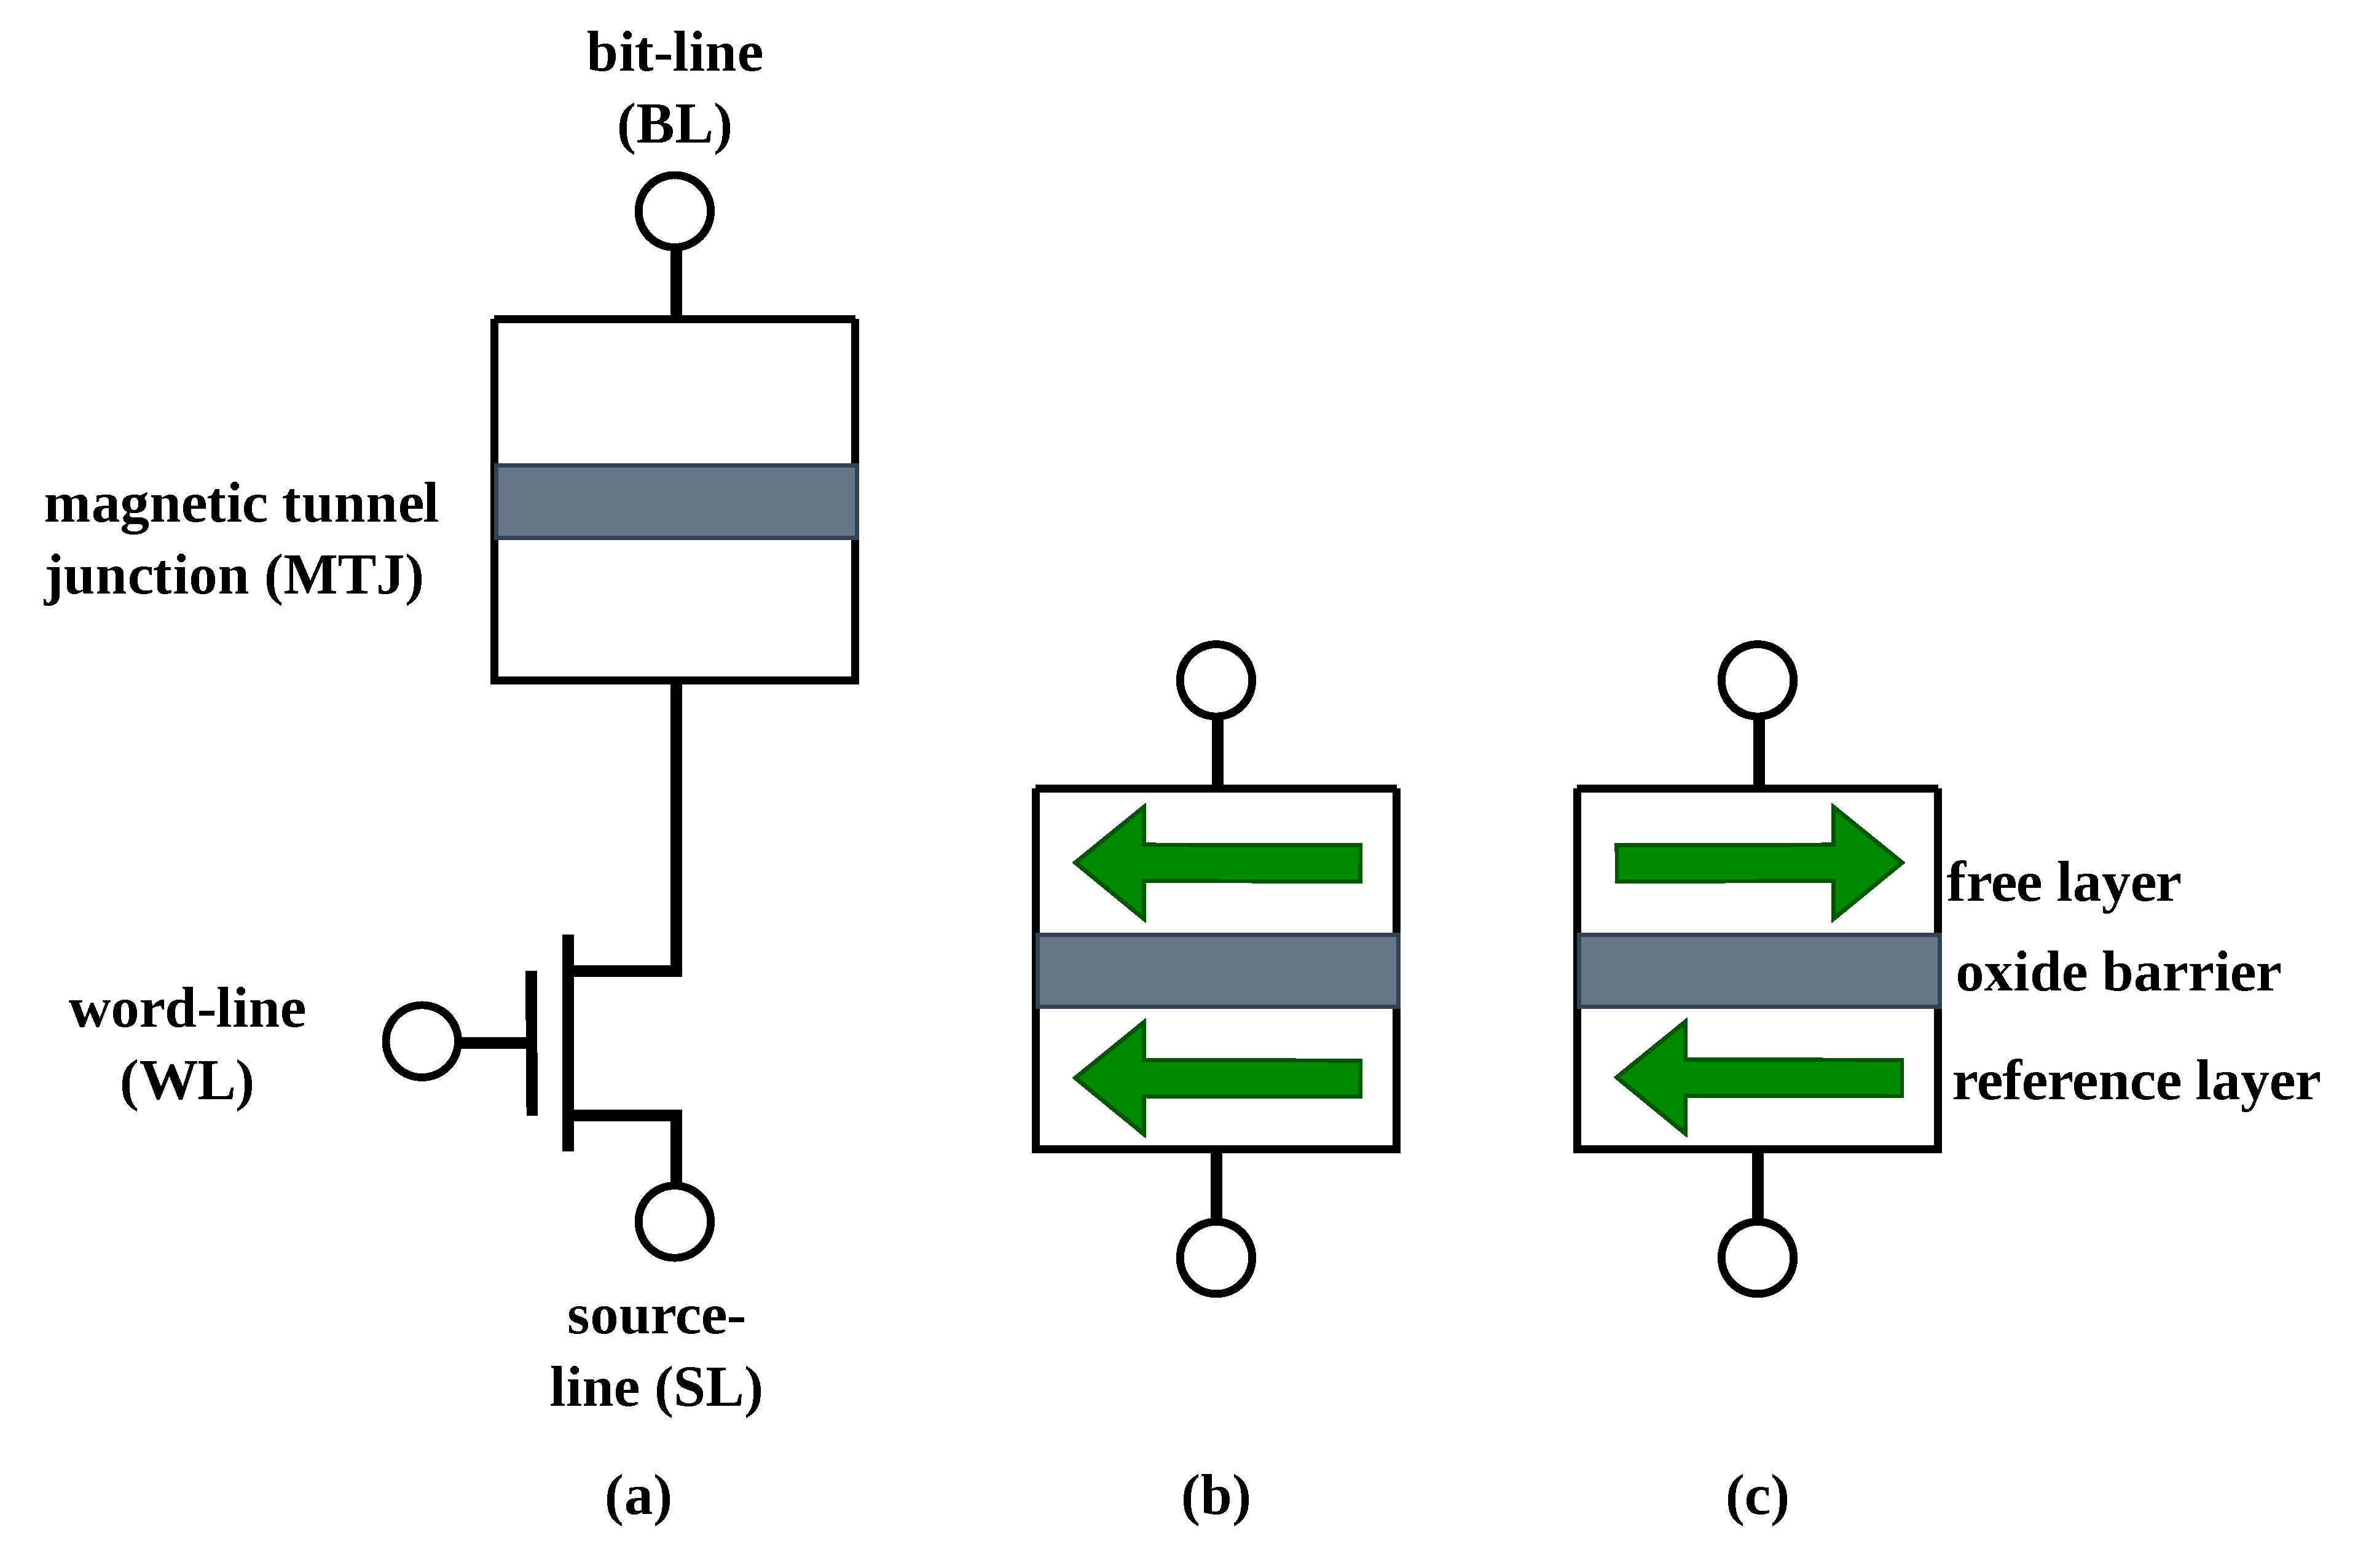
\includegraphics [scale=0.12]{fig/01.drawio.pdf}}
% \caption{STT-MRAM structure. (a) STT-MRAM cell. (b) Parallel (P) state. (c) Antiparallel (AP) state \cite{nguyen2023improving}.}
% \label{figcell}
% \end{figure}

% \begin{figure}[t]
% \centerline{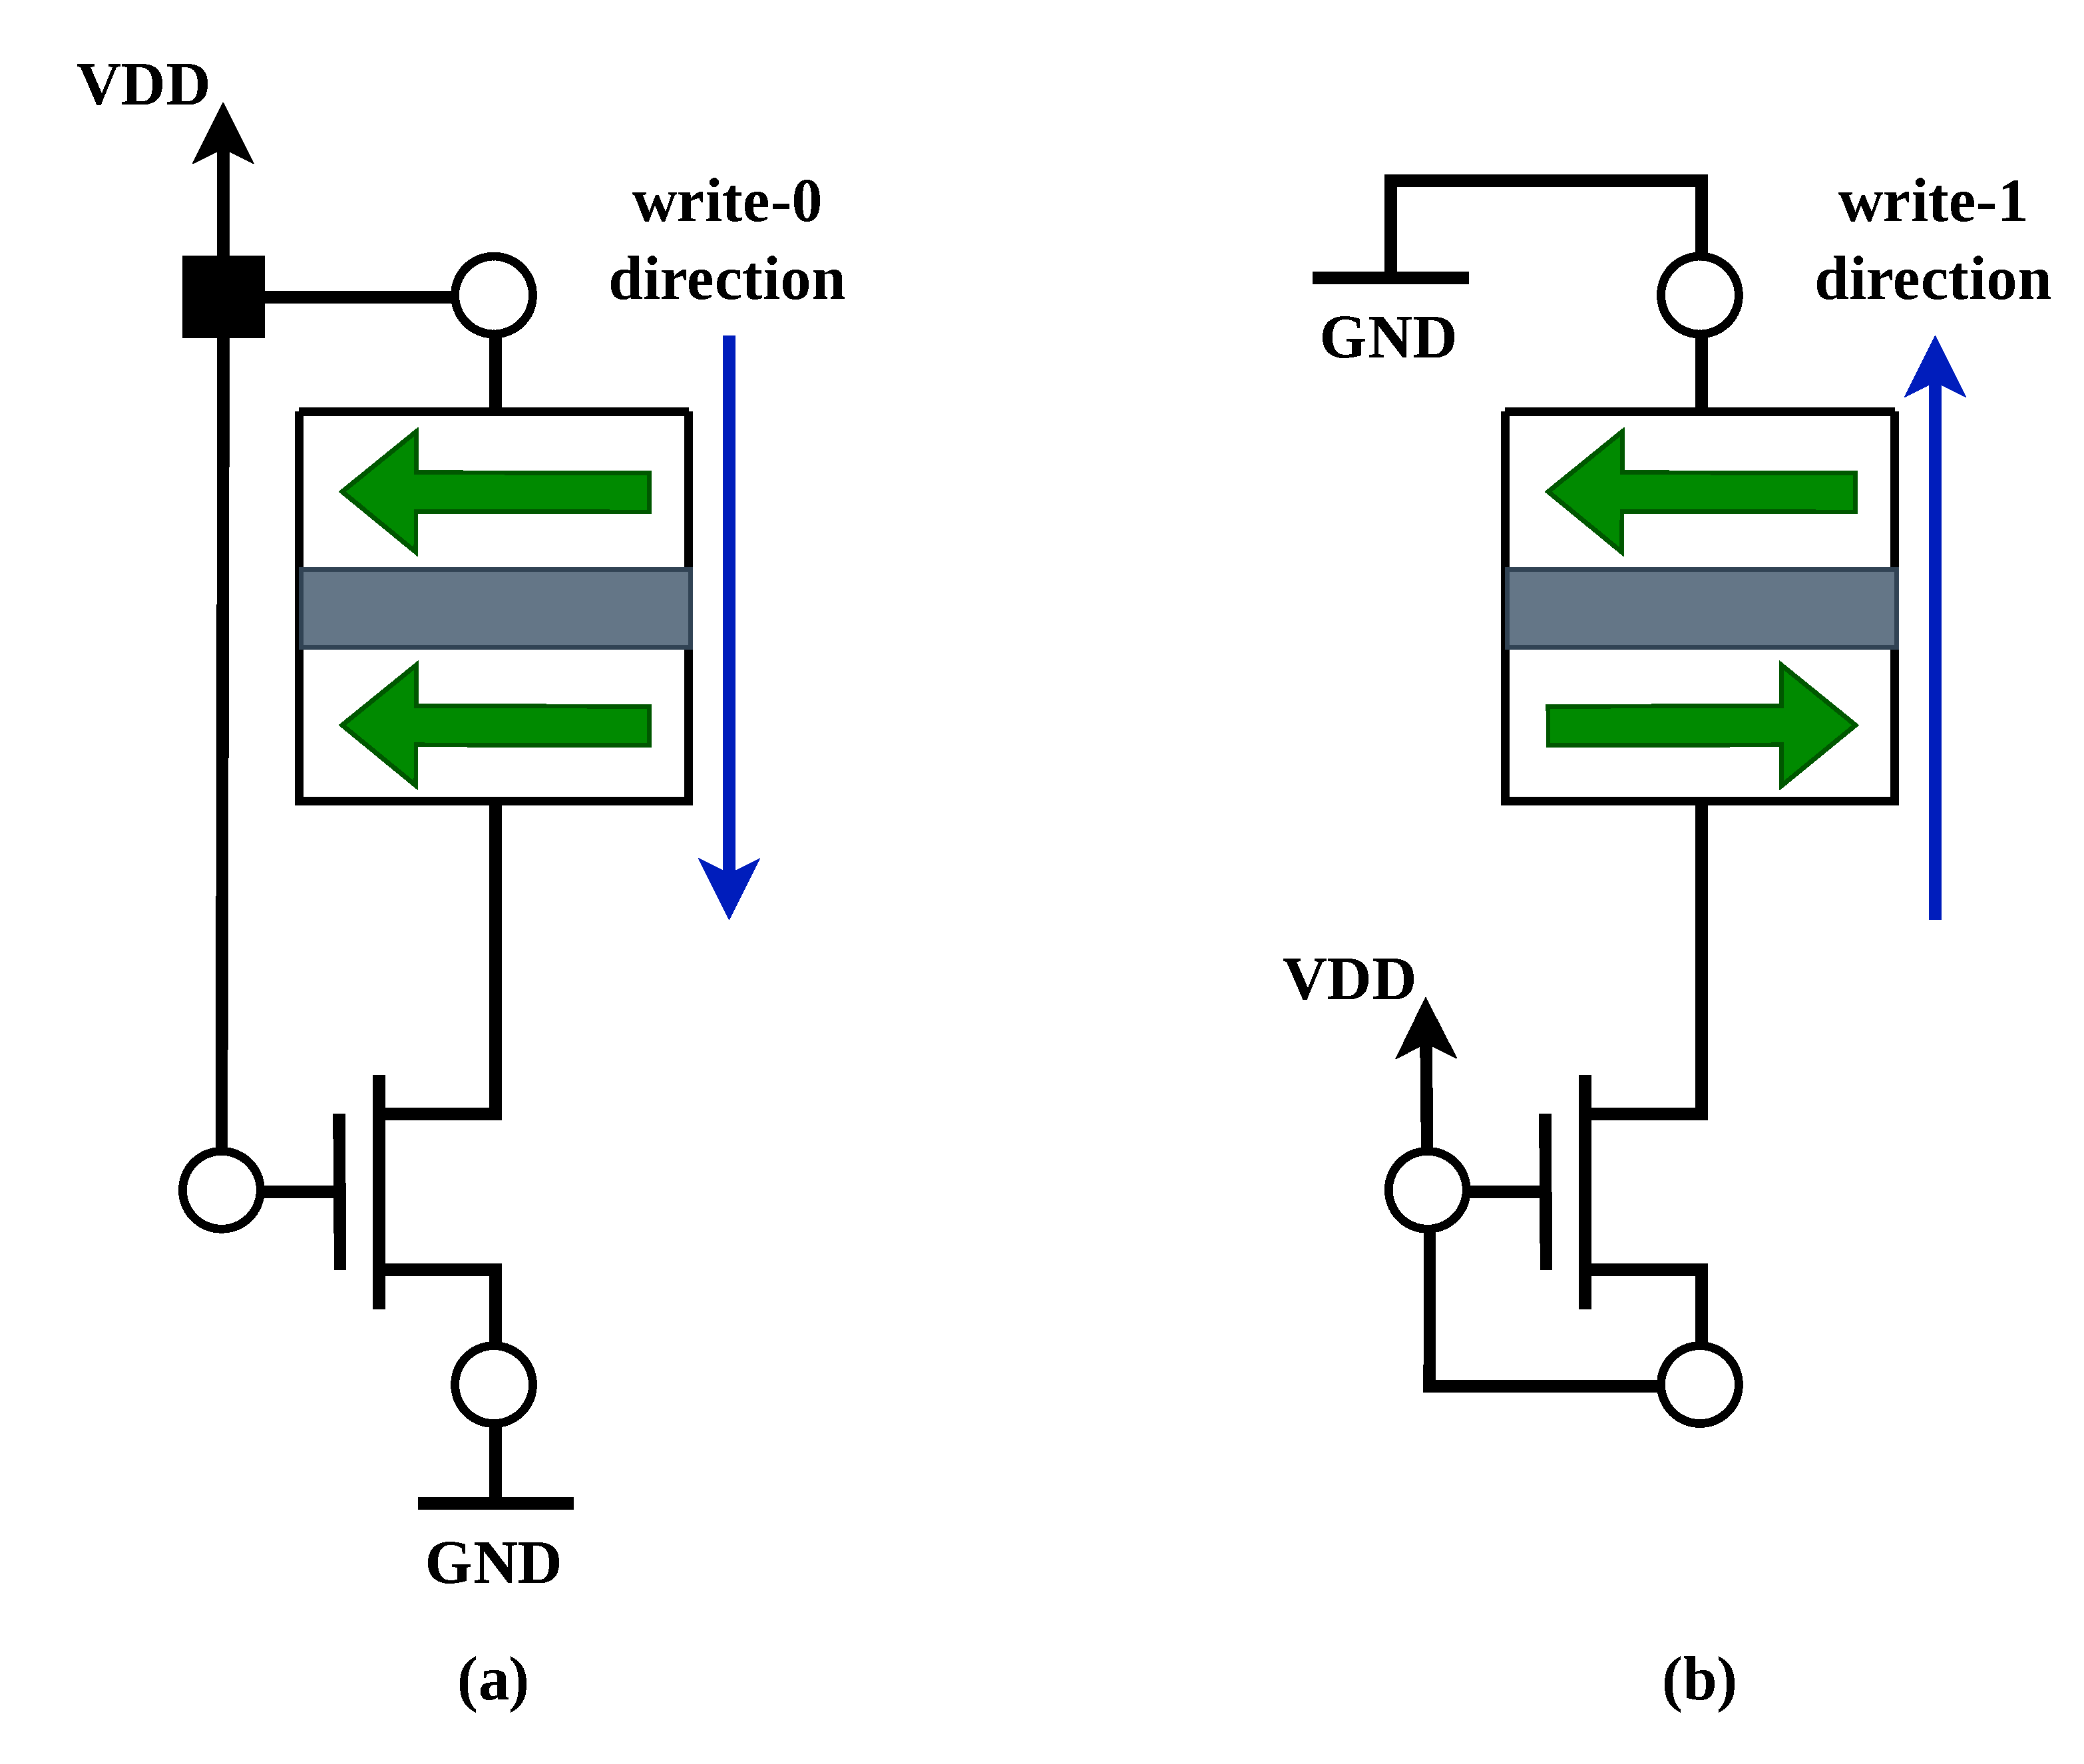
\includegraphics [scale=0.12]{fig/03.drawio.pdf}}
% \caption{Writing process in STT-MRAM. (a) Bit-0 writing process. (b) Bit-1 writing process \cite{nguyen2021design}.}
% \label{figwriteread}
% \end{figure}

The write operation exhibits strong asymmetry \cite{nguyen2021design}. Writing logic '0' switches the MTJ to the P state, whereas writing logic '1' switches it to the AP state by reversing the current direction. Because switching to the AP state requires higher switching energy and a longer switching time, the $(0 \rightarrow 1)$ write-error probability can be up to three orders of magnitude higher than that of the $(1 \rightarrow 0)$ transition, making write reliability a critical challenge in STT-MRAM.

During the read operation, a small sensing current is applied through the MTJ, and a sense amplifier compares the measured resistance with a reference threshold to determine the stored bit. Read reliability is mainly determined by the tunneling magnetoresistance (TMR) ratio, where a larger TMR provides a wider sensing margin and reduces read decision errors \cite{nguyen2021design}.

\subsection{Cascaded channel model}

To evaluate the proposed decoding scheme, this paper adopts the cascaded STT-MRAM channel model proposed in \cite{cai2017cascaded}, which captures the dominant write- and read-error mechanisms.

Let $P_1$ and $P_0$ denote the write-error probabilities for writing logic 1' (physical $0\!\rightarrow\!1$ switching) and logic 0' (physical $1!\rightarrow!0$ switching), respectively, and let $P_r$ denote the read-disturb probability. Owing to the asymmetric switching behavior of MTJs, $P_1$ is typically much larger than $P_0$ \cite{nguyen2021design}. The cascaded model comprises three components: a binary asymmetric channel (BAC) representing asymmetric write failures, a Z channel (ZC) modeling read disturbance, and a Gaussian mixture channel (GMC) describing read-decision errors. The BAC uses crossover probabilities $P_0/2$ and $P_1/2$ for target bits 0 and 1, respectively, where the factor $1/2$ accounts for the equiprobable previous cell state. In the GMC, the resistance distributions of logic '0' and logic '1' are modeled as $R_0\sim\mathcal{N}(\mu_0,\sigma_0^2)$ and $R_1\sim\mathcal{N}(\mu_1,\sigma_1^2)$, respectively.

% \begin{figure}[!t]
% \centering
% 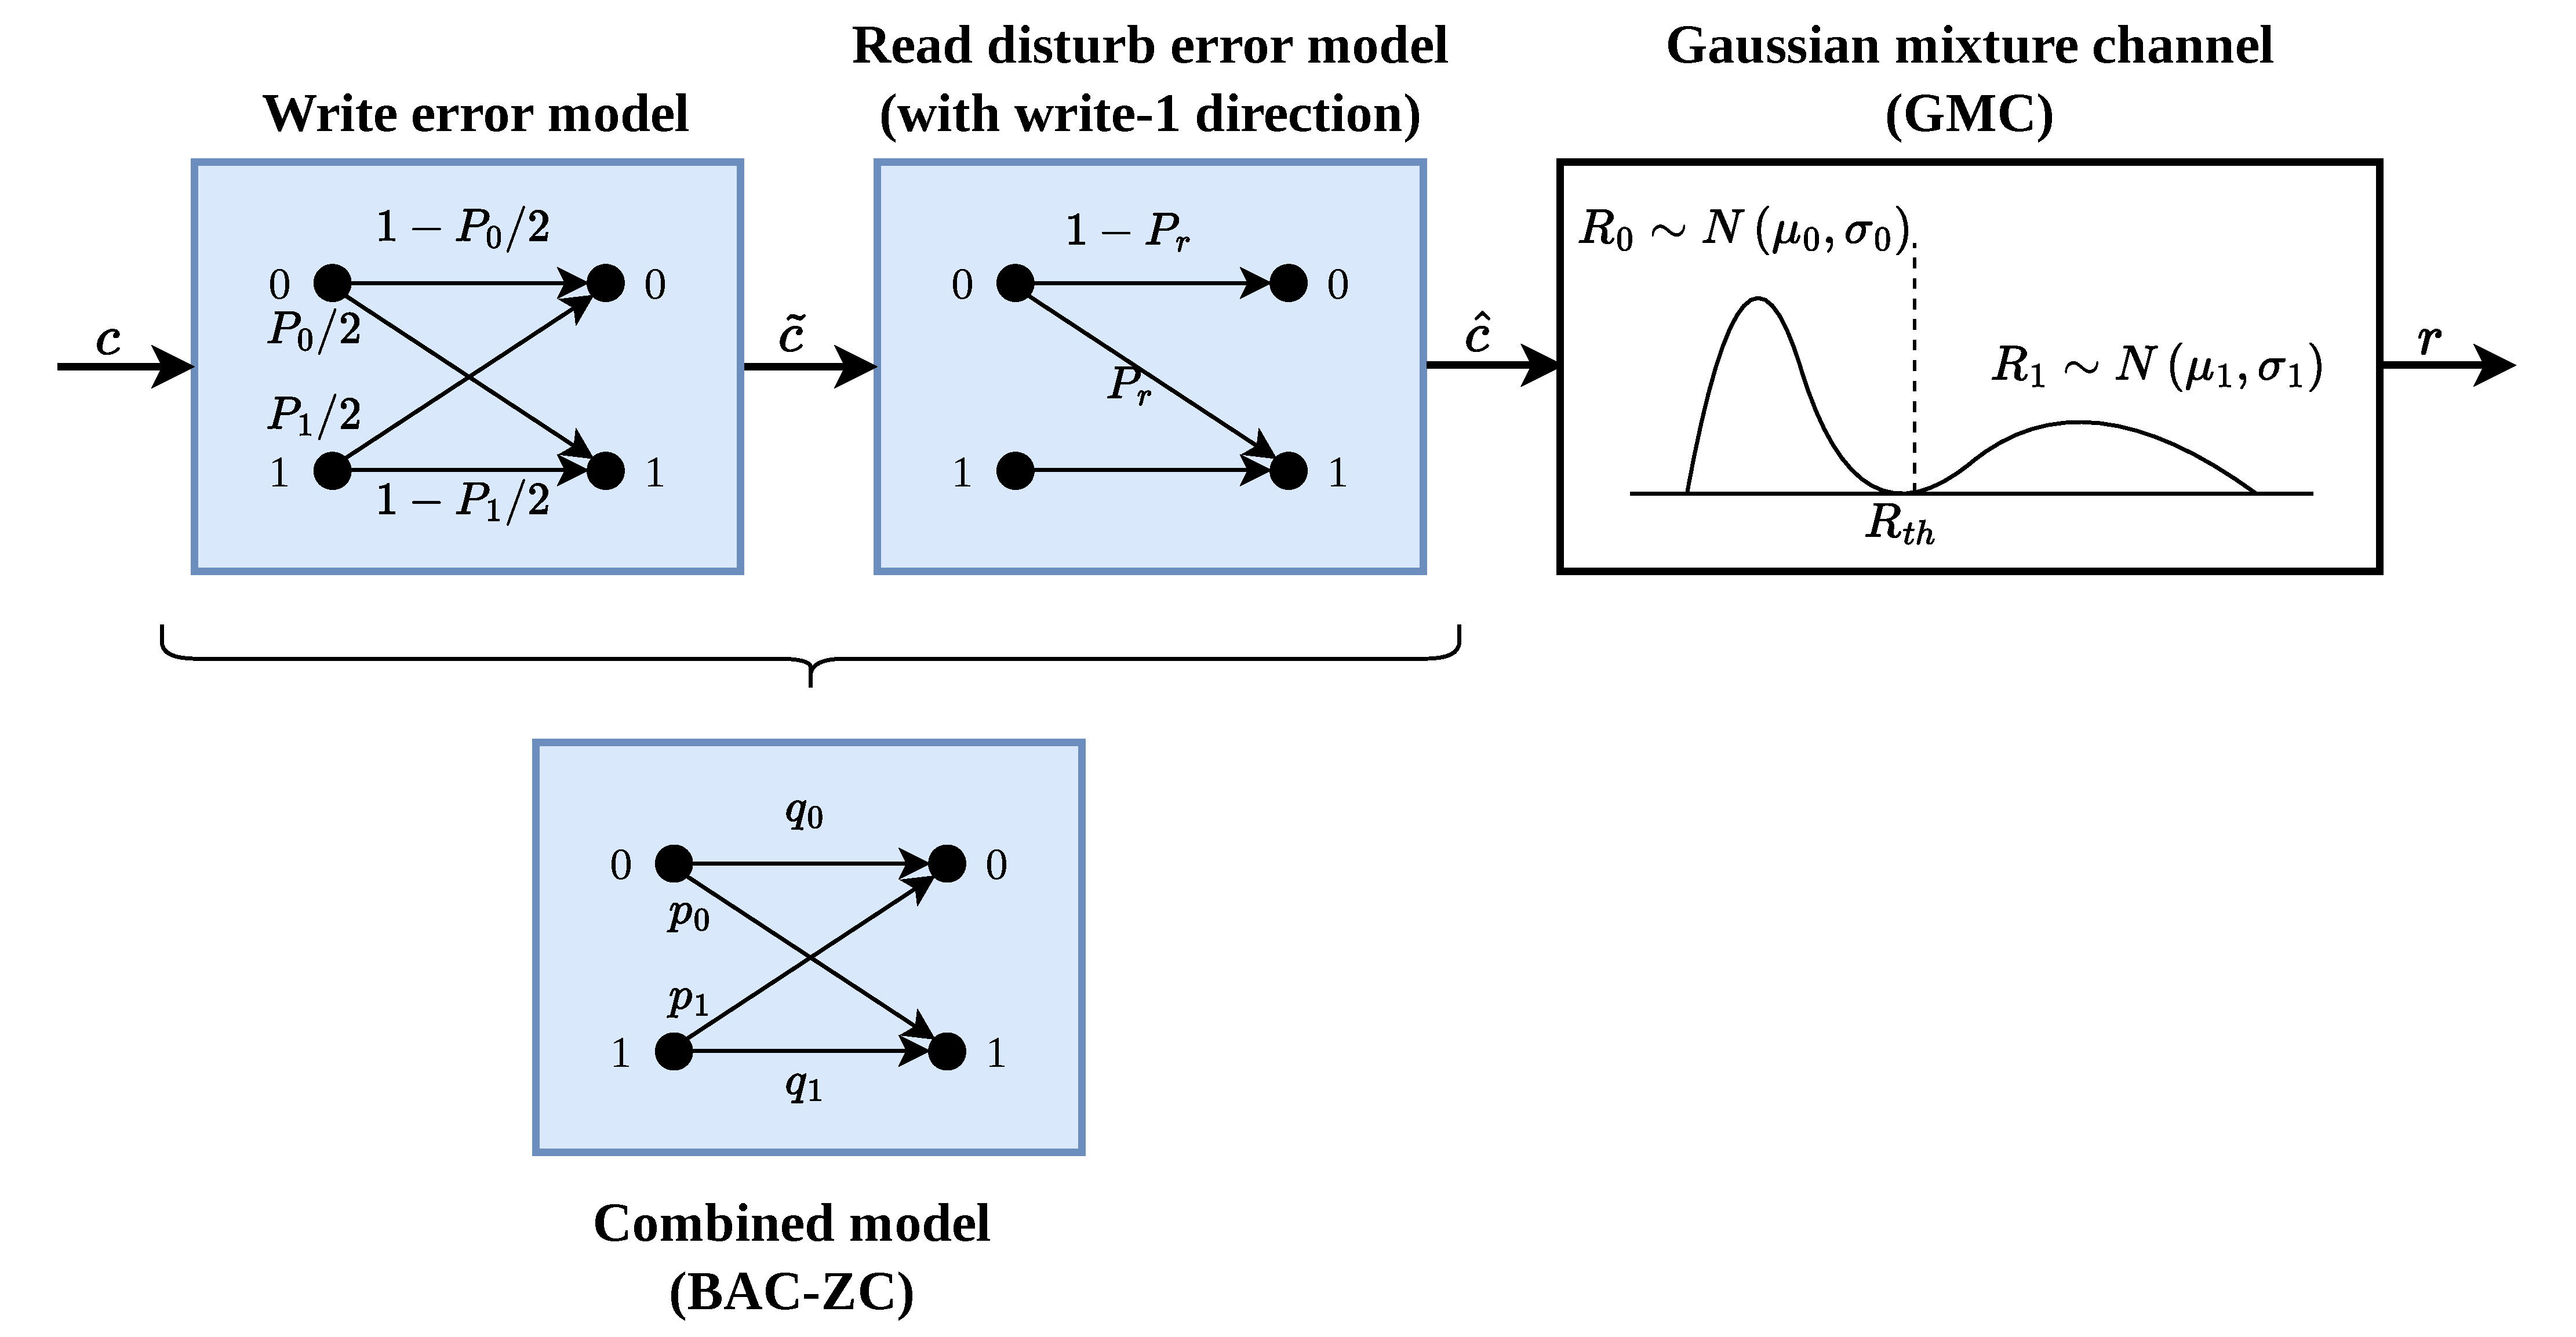
\includegraphics[width=\columnwidth]{fig/04_v2.drawio.pdf}
% \caption{Cascaded STT-MRAM channel model under the write-1 operation \cite{cai2017cascaded}.}
% \label{fig3}
% \end{figure}

For analysis, the BAC and ZC are combined into an equivalent BAC-ZC channel with transition probabilities
%
\begin{equation}
\begin{aligned}
p_0 &= \frac{P_0}{2} + \left(1 - \frac{P_0}{2}\right) P_r, \quad
q_0 = \left(1 - \frac{P_0}{2}\right)(1 - P_r), \\
p_1 &= \frac{P_1}{2} + (1 - P_r), \quad
q_1 = \left(1 - \frac{P_1}{2}\right) + \frac{P_1}{2} P_r.
\end{aligned}
\end{equation}

where $p_0$ and $p_1$ denote the probabilities of the $0\rightarrow 1$ and $1\rightarrow 0$ transitions, respectively, while $q_0$ and $q_1$ denote the probabilities of correct transitions.

\section{Proposed SLNN-Assisted Reliability Enhancement Framework}
\label{section_design}

\subsection{System Model}
Fig.~\ref{figsystem} illustrates the proposed SLNN-assisted decoding framework for the 7/9-rate sparse code. At the transmitter, the user data $u$ is encoded into a sparse codeword $c$, where each 7-bit information word is mapped to a 9-bit codeword with a Hamming weight of either 2 or 4 \cite{nguyen2021design}. This low-weight representation reduces the number of stored `1' bits and consequently the occurrence of error-prone $(0 \rightarrow 1)$ write transitions.

The encoded codeword is transmitted through the cascaded STT-MRAM channel, which captures asymmetric write failures, read disturbance, and read-decision errors. At the receiver, the noisy observation $r$ is directly processed by the proposed SLNN-based decoder, which exploits the soft information of the received signal to estimate the transmitted codeword and recover the user data $\hat{u}$.

Unlike the conventional maximum-likelihood (ML) decoder, the proposed SLNN-based decoder learns the nonlinear mapping from noisy received vectors to valid sparse codewords, thereby improving decoding accuracy while preserving the original 7/9-rate sparse coding structure. The encoding procedure is omitted for brevity and can be found in \cite{nguyen2021design}.
%
\begin{figure*}[t]
\centerline{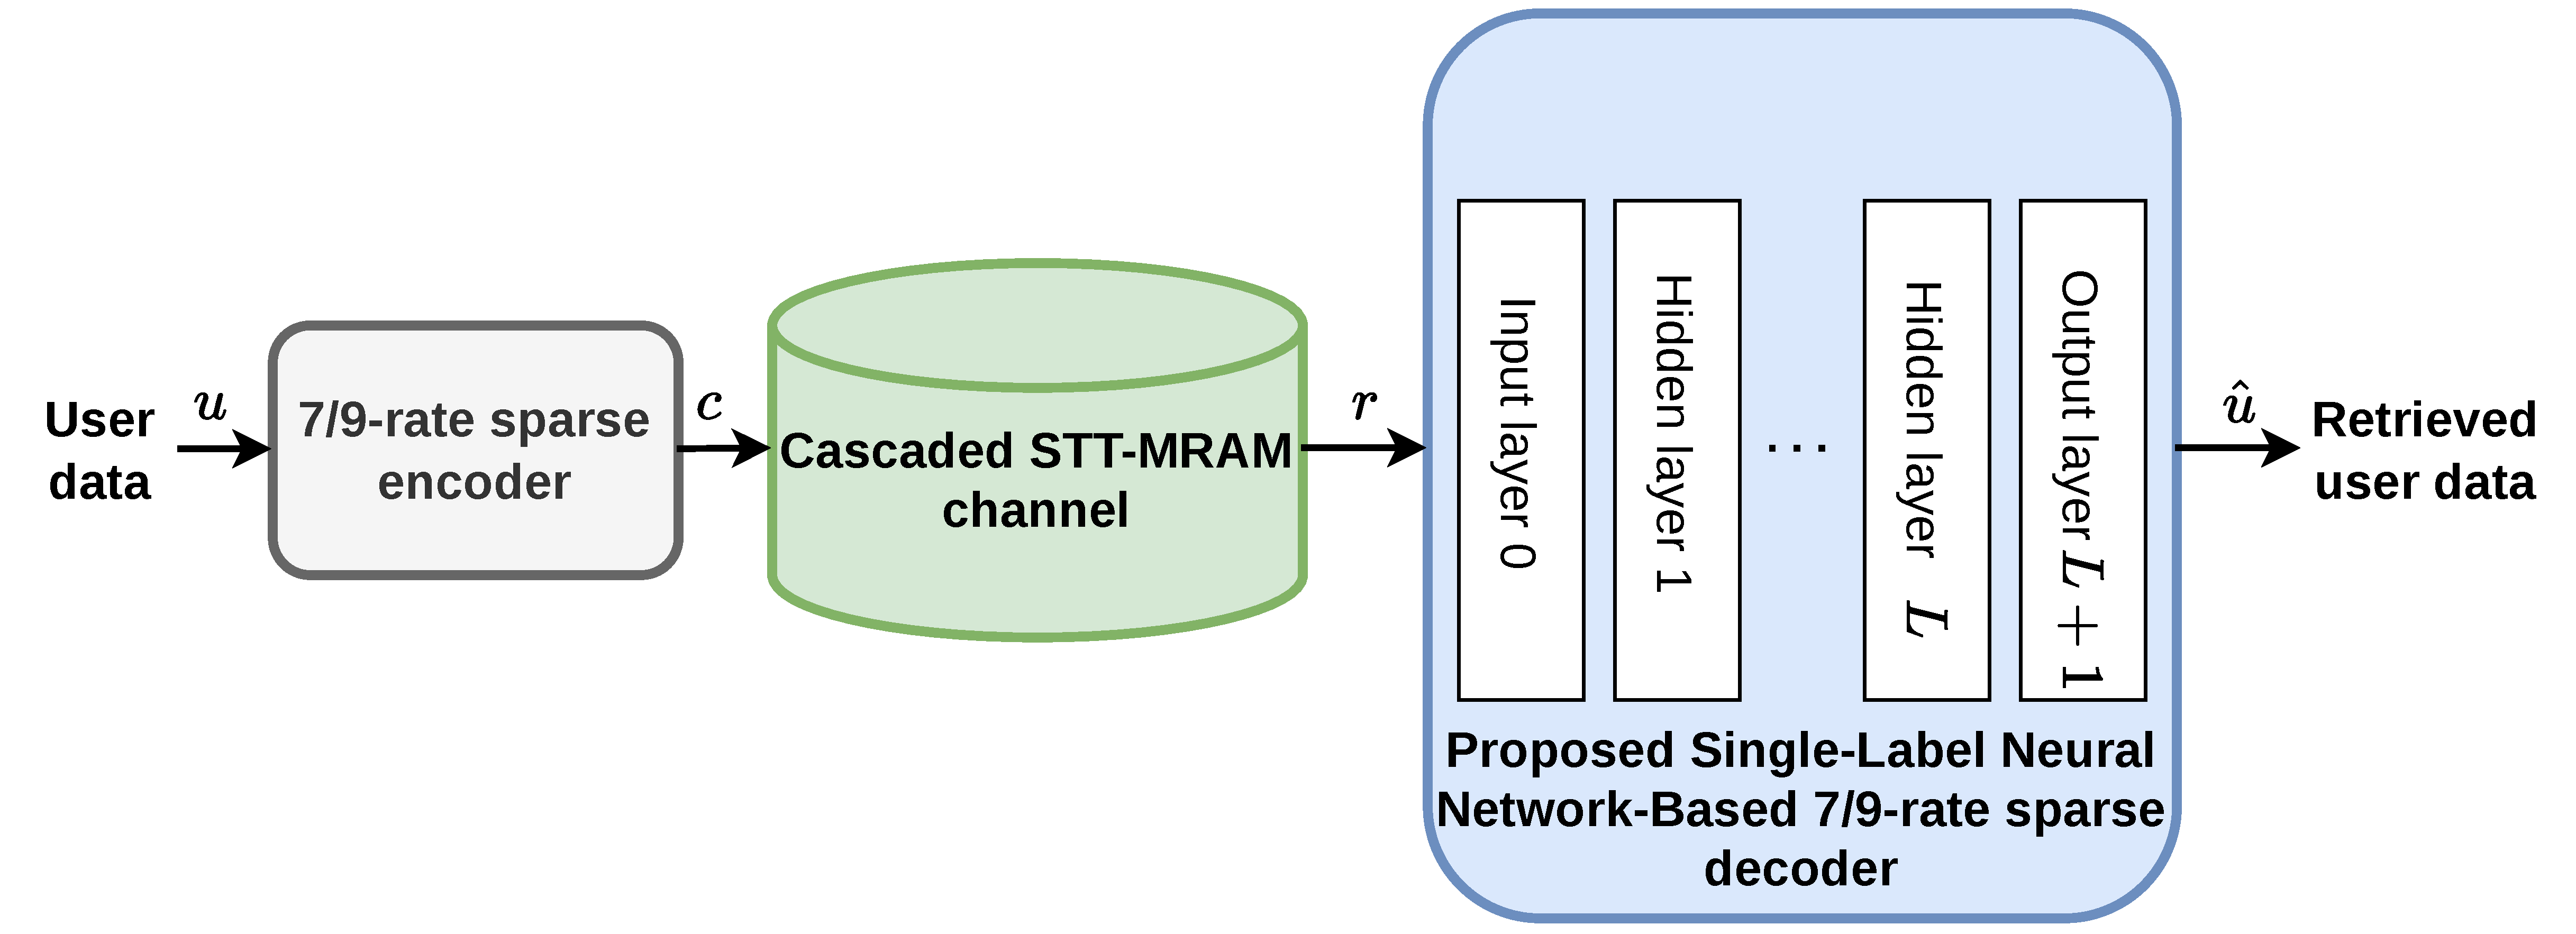
\includegraphics [scale=0.15]{fig/figsys_02.drawio.pdf}}
\caption{Block diagram of the proposed system. The SLNN-based decoder exploits the soft information of the received signals to recover the transmitted sparse codeword over the cascaded STT-MRAM channel.}
\label{figsystem}
\end{figure*}


\subsection{Single-Label Neural Network-Based 7/9-Rate Sparse Decoder}

The 7/9-rate sparse code in \cite{nguyen2021design} maps each 7-bit information word to one of 128 valid 9-bit codewords with a Hamming weight of either 2 or 4. Accordingly, sparse decoding is formulated as a 128-class single-label classification problem, where each codeword is assigned a unique class label represented by one-hot encoding during supervised training.

\begin{figure*}[t]
\centerline{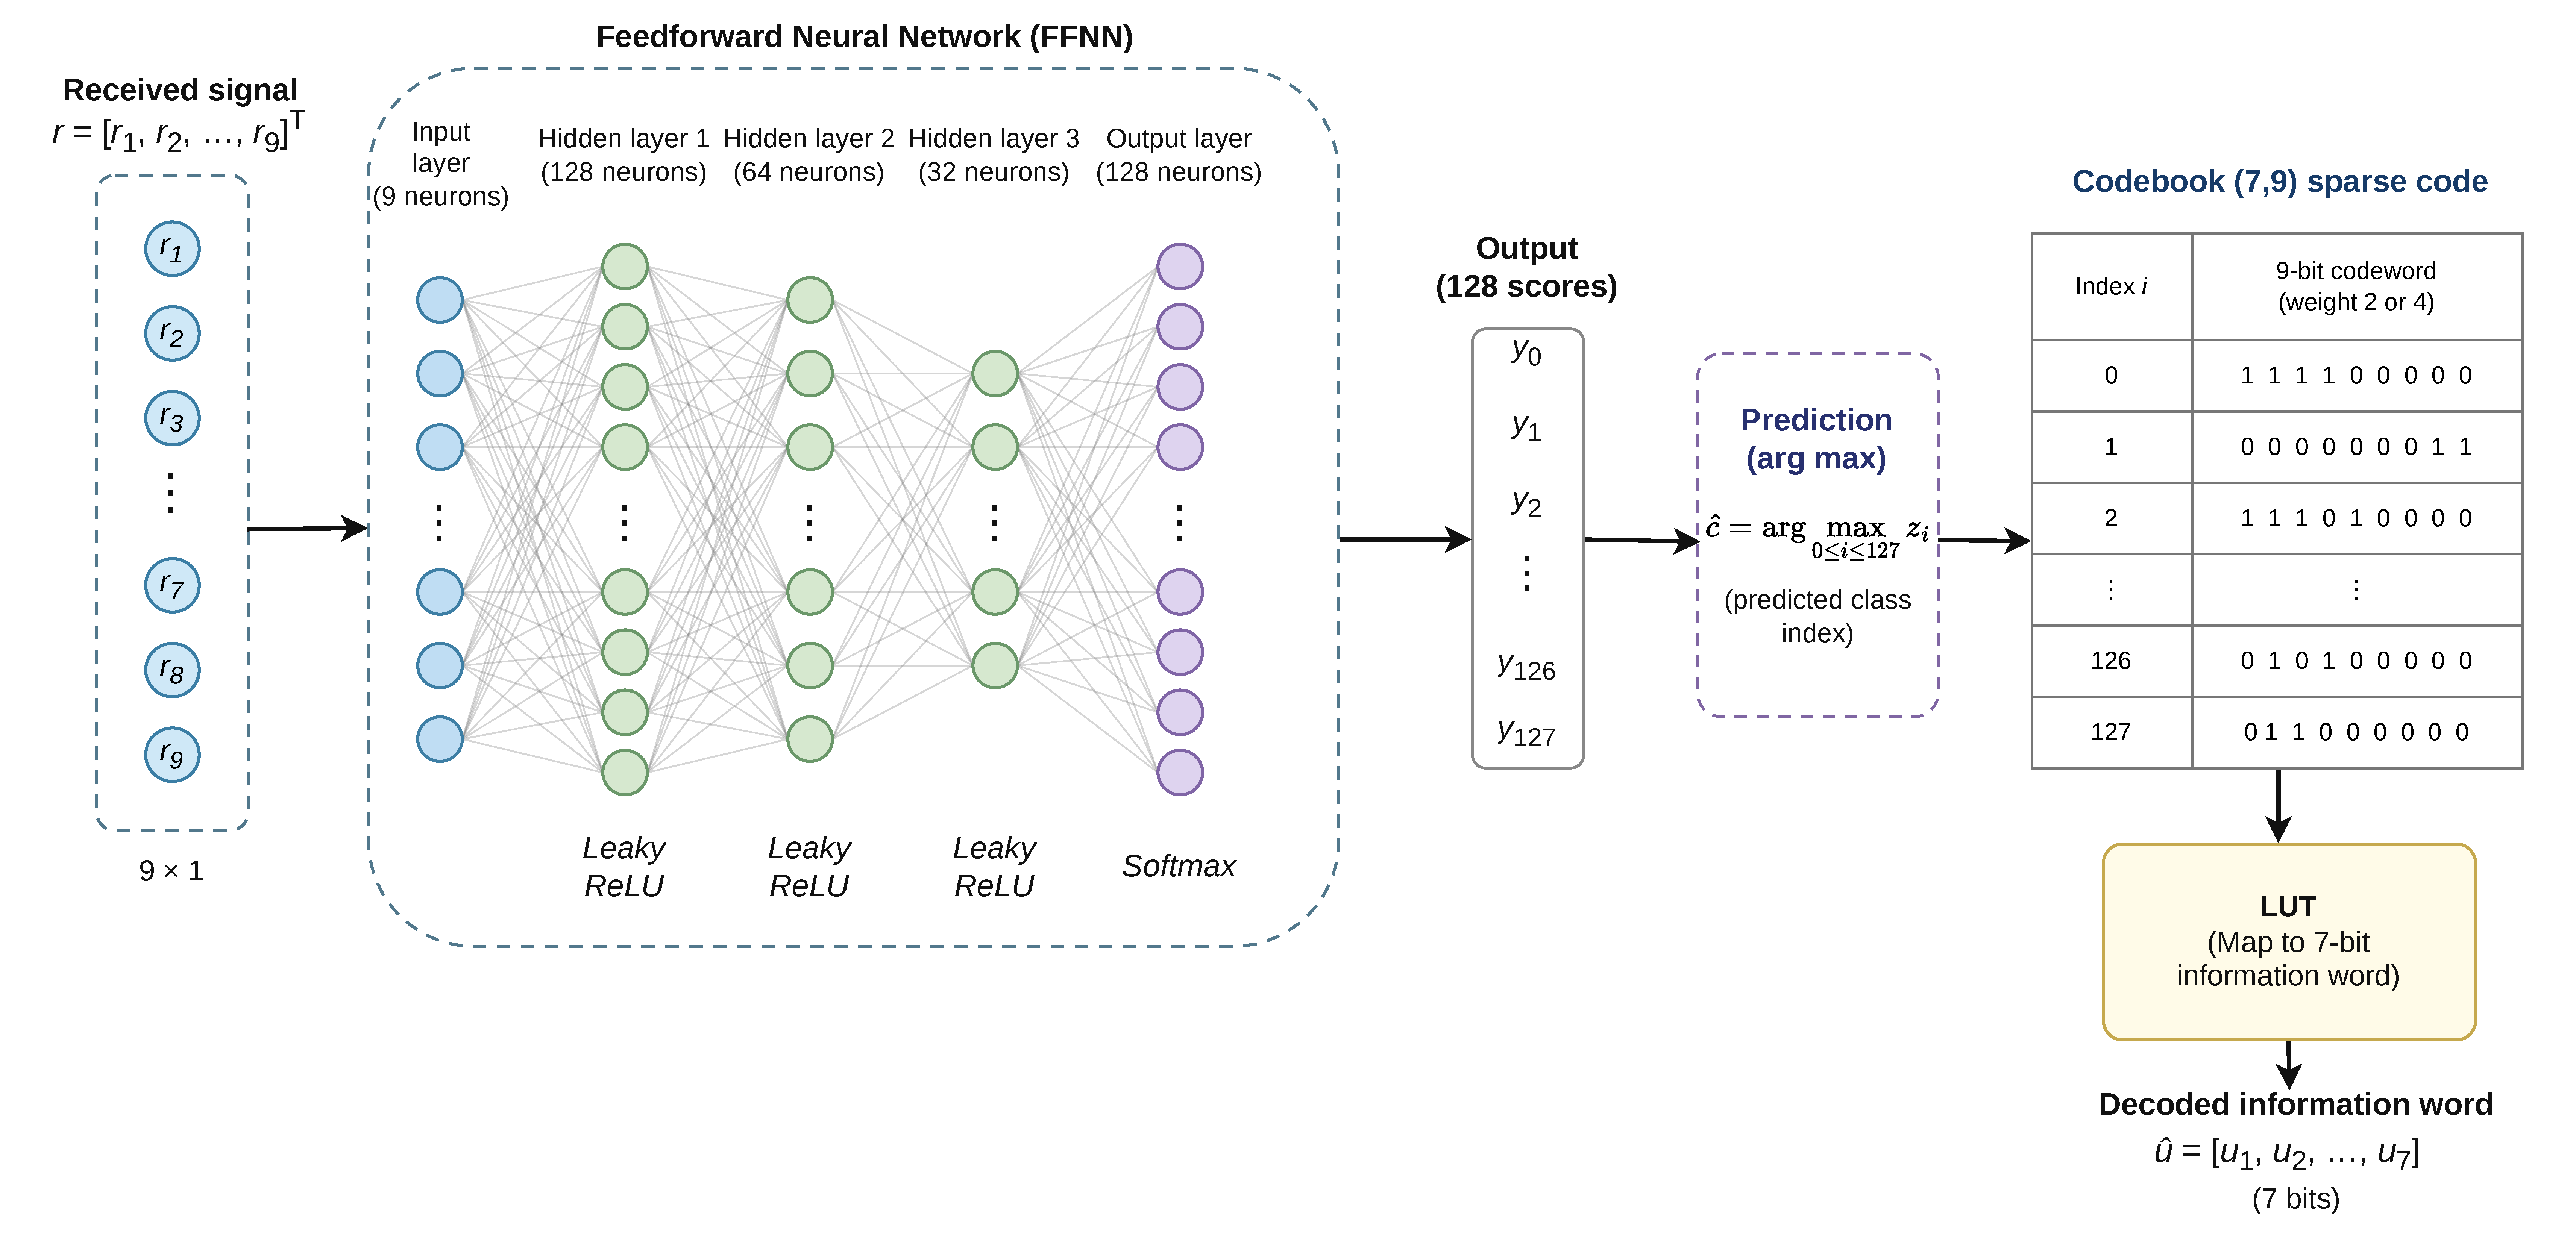
\includegraphics [scale=0.15]{fig/ffnn-decoder-diagram.drawio.pdf}}
\caption{Block diagram of the proposed single-label neural network (SLNN)-based decoder for the (7,9)-rate sparse code.}
\label{fig:SLNN_decoder}
\end{figure*}

Fig.~\ref{fig:SLNN_decoder} illustrates the proposed SLNN-based decoder. The received vector $\mathbf{r}=[r_1,r_2,\ldots,r_9]$ is fed into a feedforward neural network (FFNN), which learns the nonlinear mapping between noisy channel observations and valid sparse codewords. The output layer contains 128 neurons, each corresponding to one codeword in the sparse-code codebook. During inference, the codeword associated with the highest output probability is selected and mapped to the corresponding 7-bit information word using a look-up table (LUT).

The proposed decoder employs the FFNN architecture in \cite{gruber2017deep}, following a $9$-$128$-$64$-$32$-$128$ configuration with three hidden layers containing $128$, $64$, and $32$ neurons, respectively. Each hidden layer consists of a fully connected layer \cite{petersen2021topological}, followed by Batch Normalization \cite{ioffe2015batch} and a LeakyReLU activation function \cite{xu2015empirical}. Batch Normalization introduces two learnable parameters, $\gamma$ and $\beta$, to rescale and shift the normalized activations. The LeakyReLU activation function is defined as
%
\begin{equation}
\phi(x)=
\left\{
\begin{array}{ll}
x, & x \ge 0,\\
\alpha x, & x < 0.
\end{array}
\right.
\label{eq:leakyrelu}
\end{equation}
where $\alpha=0.01$ is the negative slope coefficient \cite{xu2015empirical}. The 128 neuron output layer produces the logits
$\mathbf{z}=[z_0,z_1,\ldots,z_{127}]$, which are converted
into class probabilities using the Softmax function
\cite{martins2016softmax}, the predicted codeword class is obtained as
%
\begin{equation}
\hat{c}
=
\arg\max_{0\leq i\leq127}\operatorname[{softmax}(\mathbf{z})_i],\qquad i=0,1,\ldots,127.
\end{equation}
%
where $\hat{c}$ denotes the predicted class label of the decoded sparse codeword.

The total number of trainable parameters is given by
%
\begin{equation}
N_{\mathrm{param}}
=
\sum_{l=1}^{L}
(n_{l-1}n_l+n_l)
+
2\sum_{l=1}^{L-1}n_l,
\label{eq:param}
\end{equation}
%
where the first term accounts for the weights and biases of the fully connected layers, and the second term represents the learnable Batch Normalization parameters. For the adopted $9$-$128$-$64$-$32$-$128$ architecture, the proposed SLNN contains 16,288 trainable parameters.

Following the data generation strategy in \cite{bennatan2018deep}, the training dataset is generated by Monte Carlo simulation of the STT-MRAM channel. Each valid 9-bit sparse codeword is transmitted through the channel to produce a noisy received vector, which serves as the network input, while the corresponding codeword index is used as the target class label.

% The network input is given by
% %
% \begin{equation}
%     \mathbf{y}
%     =
%     [y_1,y_2,\ldots,y_9]
%     \in\mathbb{R}^{9},
%     \label{eq:received_vector}
% \end{equation}
% %
% where the nine elements are the read values obtained at the
% output of the STT-MRAM channel. The received vector is directly
% normalized without applying a hard-threshold decision:
% %
% \begin{equation}
%     \widetilde{\mathbf{y}}
%     =
%     \frac{\mathbf{y}-1.5}{0.5}.
%     \label{eq:input_normalization}
% \end{equation}

% The neural decoder employs a
% $9$-$128$-$64$-$32$-$128$ architecture, in which the
% $128$-$64$-$32$ hidden-layer configuration follows the neural
% decoder studied in \cite{gruber2017deep}. The three hidden
% layers perform the transformations $9\rightarrow128$,
% $128\rightarrow64$, and $64\rightarrow32$, respectively.
% Each linear layer is followed by batch normalization and a
% LeakyReLU activation function with a negative slope of $0.01$.
% The final layer performs the $32\rightarrow128$ transformation
% and produces 128 logits. No batch normalization or LeakyReLU
% activation is applied to this layer.

% Given the logit vector $\mathbf{z}\in\mathbb{R}^{128}$, the
% class probabilities are determined using the softmax function.
% The decoded class is selected as
% %
% \begin{equation}
%     \widehat{c}
%     =
%     \underset{c\in\{0,\ldots,127\}}
%     {\operatorname{arg\,max}}
%     \left[
%         \operatorname{softmax}(\mathbf{z})
%     \right]_{c}.
%     \label{eq:class_decision}
% \end{equation}
% %
% Finally, the predicted class index $\widehat{c}$ is converted
% into its corresponding 7-bit information word using the
% decoding lookup table. During training, each sample is assigned
% a single label, and the cross-entropy loss is computed directly
% from the 128 output logits.


% \begin{table}[tb]
% \centering
% \caption{Summary of the considered BCH–sparse concatenated coding schemes and their corresponding overall coding rates.}
% \label{tab4}
% \renewcommand{\arraystretch}{1.2}
% \begin{tabular}{|c|c|c|}
% \hline
% No. 
% & Coding scheme 
% & Overall rate 
%  \\
% \hline\hline

% 1 & BCH(127,106,3) + 7/9-rate sparse code
% & 0.649 
%  \\ \hline

% 2 & BCH(127,99,4) + 7/9-rate sparse code
% & 0.606
%  \\ \hline

% 3 & BCH(127,106,3) + 4/9-rate sparse code
% & 0.371
%  \\ \hline

% 4 & BCH(127,99,4) + 4/9-rate sparse code 
% & 0.346
%  \\
% \hline
% \end{tabular}
% \end{table}

\section{SIMULATION RESULTS AND DISCUSSION} \label{section_simulation}

In this section, the bit error rate (BER) and frame error rate (FER) performances of the proposed scheme are evaluated through Monte Carlo simulations. For each operating point, independent information frames were generated, encoded, transmitted through the STT-MRAM channel, and decoded using the corresponding decoding scheme. The BER was obtained by comparing the decoded information bits with the transmitted bits, while the FER was defined as the ratio of incorrectly decoded frames to the total number of transmitted frames. To ensure statistically reliable BER and FER estimates, each simulation was terminated after processing at least $10^6$ information bits.


\subsection{Simulation setup}

This subsection evaluates the BER and FER performance of the considered coding schemes as functions of the coefficient of variation $\sigma_0/\mu_0$ and the write-error probability $P_1$, following the simulation methodology in \cite{an2025sparse,nguyen2021design}. The simulation parameters are adopted from the experimentally validated STT-MRAM model in \cite{cai2017cascaded,zhang2011stt}, using a 45-nm predictive technology model (PTM)-based STT-MRAM cell. The mean resistances of the low- and high-resistance states are set to $1~\mathrm{k}\Omega$ and $2~\mathrm{k}\Omega$, respectively, with identical coefficients of variation, i.e., $\sigma_0/\mu_0=\sigma_1/\mu_1$.

The parameter $\sigma_0/\mu_0$ characterizes resistance variation during read operations, where a larger value results in more severe read decision errors. In contrast, $P_1$ denotes the probability of a bit-1 write error caused by incomplete switching or read-disturb-induced state changes. Since $P_0$ and $P_r$ are typically much smaller than $P_1$ (i.e., $P_0,P_r\ll P_1$), the overall BER performance is mainly dominated by $P_1$.



\subsection{Simulation results}


In this subsection, we compare the BER and FER performance of the proposed SLNN-based decoder with that of the conventional ML decoder for the 7/9-rate sparse code \cite{nguyen2021design}. Figures~\ref{ber_fer_vs_sigma} and \ref{ber_fer_vs_p1} present the BER and FER performance versus the coefficient of variation $(\sigma_0/\mu_0)$ and the write-error probability $(P_1)$, respectively. The results indicate that the proposed SLNN-based decoder consistently outperforms the conventional ML decoder under all simulated channel conditions. On average, the proposed decoder achieves an approximately 60\% reduction in both BER and FER, demonstrating the effectiveness of the proposed SLNN-based decoding approach.

\begin{figure}[t]
\centerline{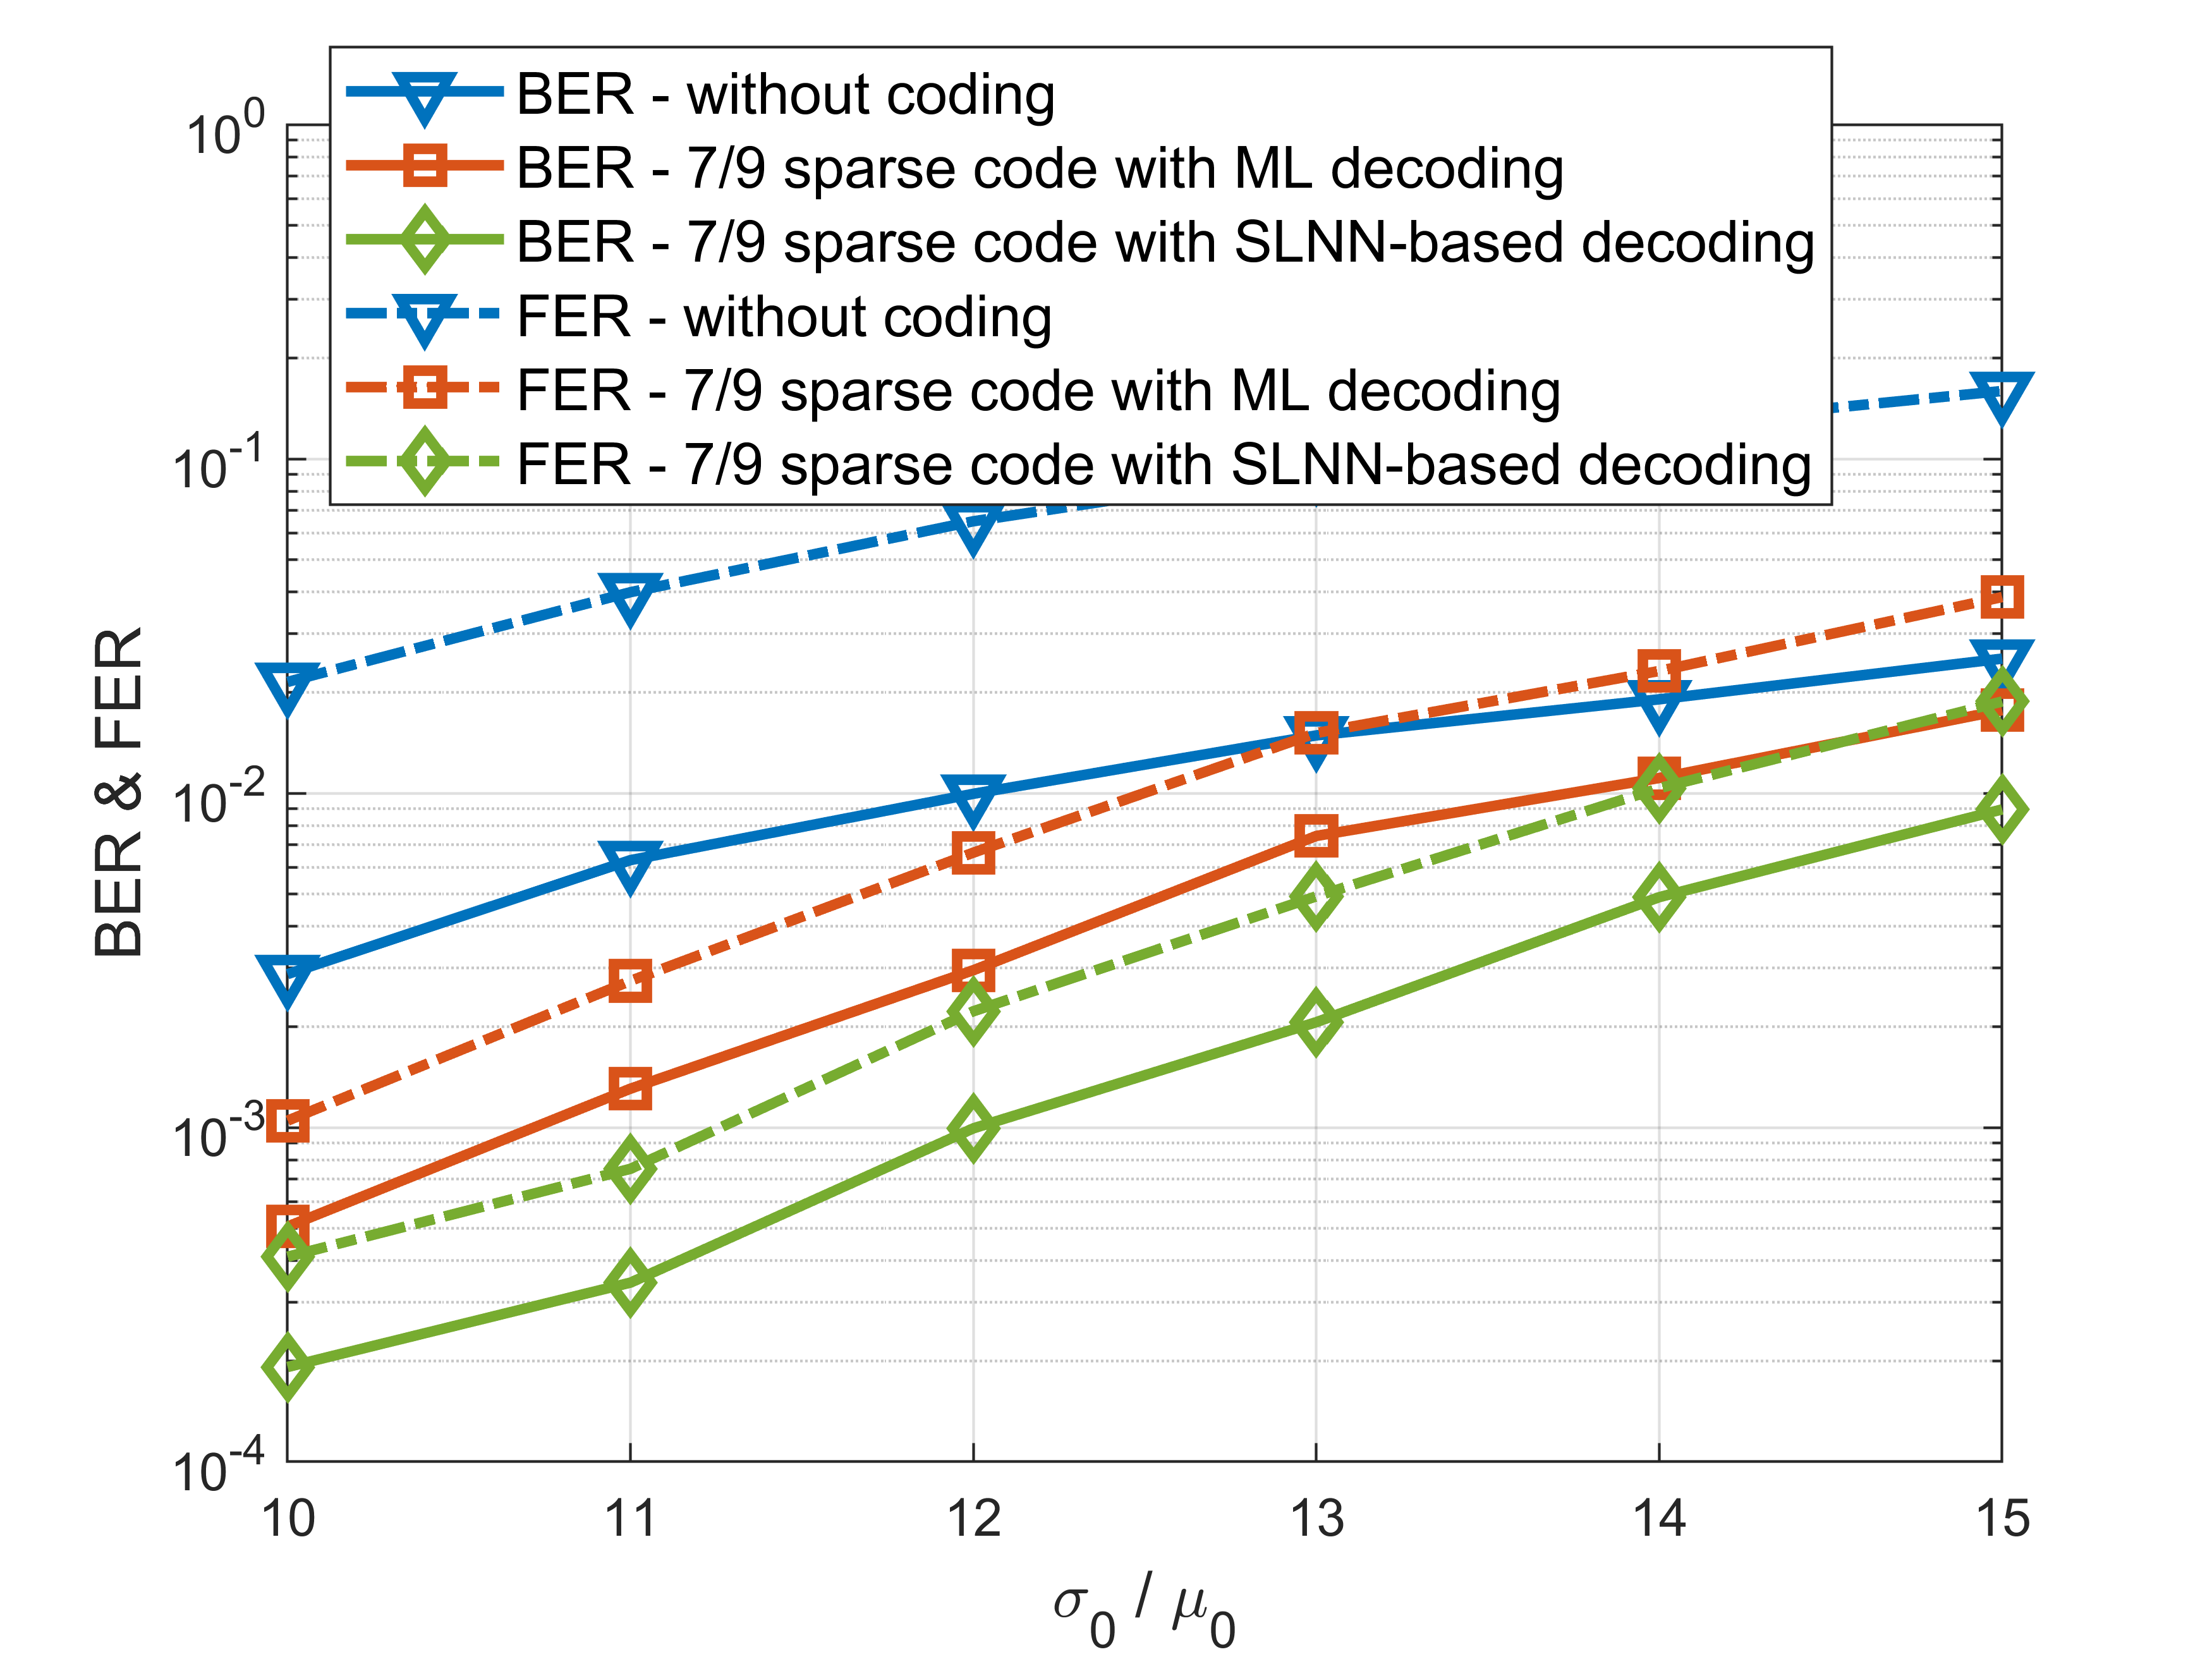
\includegraphics [scale=0.65]{fig/BER_FER_vs_sigma.png}}
\caption{Comparison of ML decoding and the proposed SLNN-based decoding for the $(7,9)$-rate sparse code in terms of BER and FER versus the coefficient of variation $(\sigma_0/\mu_0)$.}
\label{ber_fer_vs_sigma}
\end{figure}

\begin{figure}[t]
\centerline{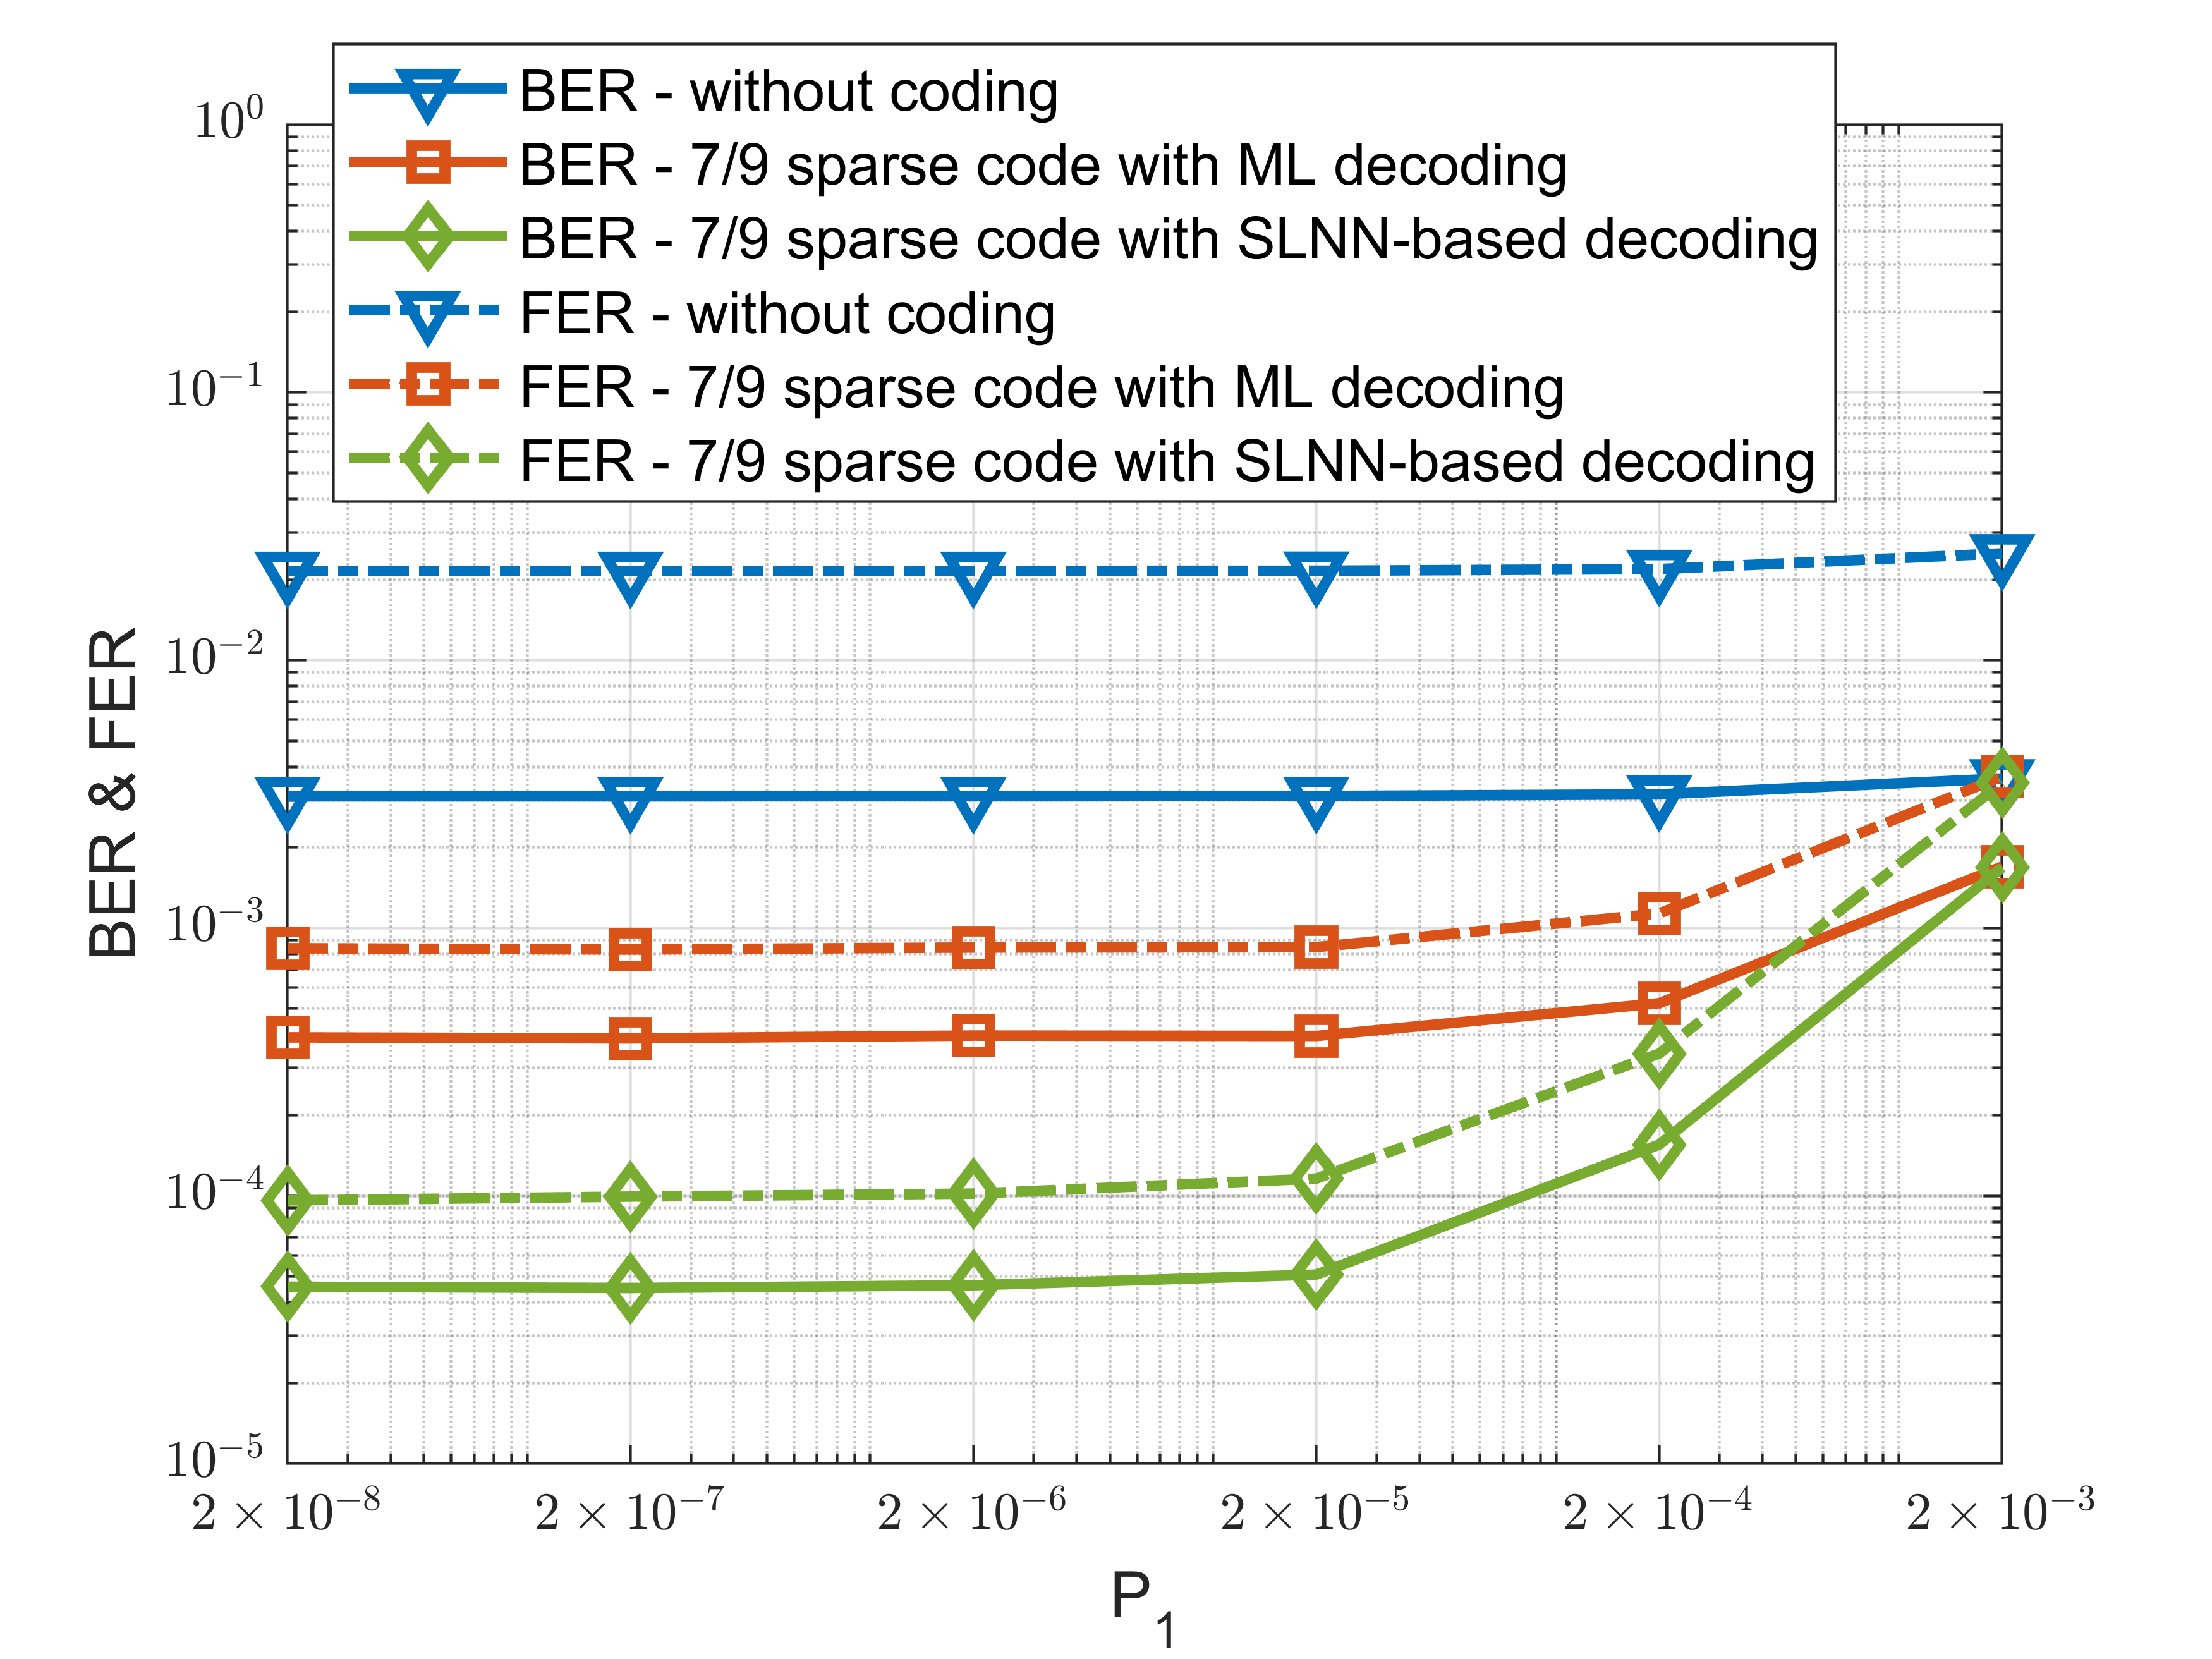
\includegraphics [scale=0.65]{fig/BER_FER_vs_p1.png}}
\caption{Comparison of ML decoding and the proposed SLNN-based decoding for the $(7,9)$-rate sparse code in terms of BER and FER versus the write error rate $(P_1)$.}
\label{ber_fer_vs_p1}
\end{figure}





\section{Conclusion} \label{section_conclusion}

This paper presented an SLNN-based decoder for the 7/9-rate sparse code to improve the reliability of STT-MRAM. By reformulating sparse decoding as a 128-class single-label classification problem, the proposed decoder directly learns the nonlinear mapping from noisy received vectors to valid sparse codewords, replacing the conventional ML decoder. A lightweight feedforward neural network architecture was adopted to realize the proposed decoder with low computational complexity. Simulation results demonstrated that the proposed decoder consistently outperformed the conventional ML decoder under various STT-MRAM channel conditions, achieving approximately 60\% average reductions in both BER and FER. These results confirm that incorporating neural learning into the sparse decoding process provides a promising approach for enhancing the reliability of STT-MRAM.

Future work will investigate the integration of the proposed SLNN-based sparse decoder with outer error-correcting codes (ECC), such as BCH and LDPC codes, to further enhance the reliability of STT-MRAM.

% \section*{Acknowledgment}







% -------------------------------------------------------------------------
\bibliographystyle{IEEEtran} % ieeetr
\bibliography{refs}





\vspace{12pt}
% \color{red}
% IEEE conference templates contain guidance text for composing and formatting conference papers. Please ensure that all template text is removed from your conference paper prior to submission to the conference. Failure to remove the template text from your paper may result in your paper not being published.

\end{document}
